\documentclass[10pt]{article}
\usepackage[usenames]{color} %used for font color
\usepackage{amssymb} %maths
\usepackage{amsmath} %maths
\usepackage[utf8]{inputenc} %useful to type directly diacritic characters
\usepackage[letterpaper, portrait, margin=.5in]{geometry}
\usepackage{graphicx,wrapfig}
\usepackage{fancyvrb}
\usepackage{booktabs}
\usepackage{multicol}
\begin{document}
\subsection*{MSDS650 Week 6 Linux Assignment - Nathan Worsham}
Exercise from http://williamjturkel.net/2013/06/15/basic-text-analysis-with-command-line-tools-in-linux/
\begin{Verbatim}[fontsize=\scriptsize]
[root@evensong Regis]# wget https://archive.org/download/thestoriesmother05792gut/stmtn10.txt
--2015-11-22 21:41:12--  https://archive.org/download/thestoriesmother05792gut/stmtn10.txt
Resolving archive.org (archive.org)... 207.241.224.2
Connecting to archive.org (archive.org)|207.241.224.2|:443... connected.
HTTP request sent, awaiting response... 302 Moved Temporarily
Location: https://ia802701.us.archive.org/8/items/thestoriesmother05792gut/stmtn10.txt [following]
--2015-11-22 21:41:13--  https://ia802701.us.archive.org/8/items/thestoriesmother05792gut/stmtn10.txt
Resolving ia802701.us.archive.org (ia802701.us.archive.org)... 207.241.228.241
Connecting to ia802701.us.archive.org (ia802701.us.archive.org)|207.241.228.241|:443... connected.
HTTP request sent, awaiting response... 200 OK
Length: 136162 (133K) [text/plain]
Saving to: ‘stmtn10.txt’

100\%[==================================================================================================================================================================>] 136,162     --.-K/s   in 0.1s    

2015-11-22 21:41:13 (1.03 MB/s) - ‘stmtn10.txt’ saved [136162/136162]

[root@evensong Regis]# ls
stmtn10.txt
[root@evensong Regis]# file stmtn10.txt
stmtn10.txt: C source, ASCII text, with CRLF line terminators
[root@evensong Regis]# head stmtn10.txt
The Project Gutenberg EBook of The Stories Mother Nature Told Her Children
by Jane Andrews

Copyright laws are changing all over the world. Be sure to check the
copyright laws for your country before downloading or redistributing
this or any other Project Gutenberg eBook.

This header should be the first thing seen when viewing this Project
Gutenberg file.  Please do not remove it.  Do not change or edit the
header without written permission.
[root@evensong Regis]# tail stmtn10.txt

[Portions of this eBook's header and trailer may be reprinted only
when distributed free of all fees.  Copyright (C) 2001, 2002 by
Michael S. Hart.  Project Gutenberg is a TradeMark and may not be
used in any sales of Project Gutenberg eBooks or other materials be
they hardware or software or any other related product without
express permission.]

*END THE SMALL PRINT! FOR PUBLIC DOMAIN EBOOKS*Ver.02/11/02*END*

[root@evensong Regis]# cp stmtn10.txt stmtn10-backup.txt
[root@evensong Regis]# ls
stmtn10-backup.txt  stmtn10.txt
[root@evensong Regis]# less -N stmtn10.txt
[root@evensong Regis]# sed '2206,2525d' stmtn10.txt > stmtn10-nofooter.txt
[root@evensong Regis]# sed '1,40d' stmtn10-nofooter.txt > stmtn10-trimmed.txt
[root@evensong Regis]# wc -l stmtn10-trimmed.txt
2165 stmtn10-trimmed.txt
[root@evensong Regis]# wc -m stmtn10-trimmed.txt
121038 stmtn10-trimmed.txt
[root@evensong Regis]# grep -n "giant" stmtn10-trimmed.txt
1115:Do you believe in giants? No, do you say? Well, listen to my story,
1138:to admit that to do it needed a giant's strength, and so they deserve
1214:giants think of doing. We have not long to wait before we shall see, and
[root@evensong Regis]# grep -E -n "(G|g)iant" stmtn10-trimmed.txt
1115:Do you believe in giants? No, do you say? Well, listen to my story,
1123:Frost Giants.
1129:present we have only to do with the Frost Giants; for I want to tell
1131:the flat earth or the rainbow bridge, yet the Frost Giants still live,
1138:to admit that to do it needed a giant's strength, and so they deserve
1143:no other rocks are near? Well, the Frost Giants carried these boulders
1157:While I thus introduce to you the Frost Giants, let me also present
1186:fitting home for the Frost Giants.
1205:the Frost Giants, and see what they are about to-day.
1214:giants think of doing. We have not long to wait before we shall see, and
1231:day be strong enough to break through the Frost Giants' dam. And the day
1262:there like boats in a stormy sea. And this is what the Frost Giants did
1311:and, so far as I know, the Frost Giants have never succeeded in touching
[root@evensong Regis]# tr -d [:punct:] < stmtn10-trimmed.txt > stmtn10-nopunct.txt
[root@evensong Regis]# less stmtn10-nopunct.txt 
[root@evensong Regis]# tr [:upper:] [:lower:] < stmtn10-nopunct.txt > stmtn10-lowercase.txt
[root@evensong Regis]# less stmtn10-lowercase.txt 
[root@evensong Regis]# tr -d '\r' < stmtn10-lowercase.txt > stmtn10-lowercaself.txt
[root@evensong Regis]# less stmtn10-lowercaself.txt 
[root@evensong Regis]# tr ' ' '\n' < stmtn10-lowercaself.txt > stmtn10-oneword.txt
[root@evensong Regis]# head stmtn10-oneword.txt 




produced
by
juliet
sutherland
charles
franks
[root@evensong Regis]# sort stmtn10-oneword.txt > stmtn10-onewordsort.txt
[root@evensong Regis]# less stmtn10-onewordsort.txt 
[root@evensong Regis]# 
[root@evensong Regis]# sort stmtn10-oneword.txt > stmtn10-onewordsort.txt
[root@evensong Regis]# uniq -c stmtn10-onewordsort.txt > stmtn10-wordfreq.txt
[root@evensong Regis]# head stmtn10-wordfreq.txt
    358 
      1 1861
      1 1865
      1 1888
      1 1894
    426 a
      1 abashed
      1 ability
      4 able
     44 about
[root@evensong Regis]# tr ' ' '\n' < stmtn10-lowercaself.txt | sort | uniq -c > stmtn10-wordfreq2.txt
[root@evensong Regis]# diff stmtn10-wordfreq.txt stmtn10-wordfreq2.txt 
[root@evensong Regis]# less stmtn10-wordfreq2.txt 
[root@evensong Regis]# 
\end{Verbatim}
Exercise from http://williamjturkel.net/2013/08/24/working-with-pdfs-using-command-line-tools-in-linux/
I first had to install several items, turns out pdftk is not compatible with Centos7.
\begin{Verbatim}[fontsize=\scriptsize]
[root@plainsong ~]# yum install openbox obconf obmenu
Loaded plugins: fastestmirror, langpacks
base                                                                                                                                                                                 | 3.6 kB  00:00:00     
extras                                                                                                                                                                               | 3.4 kB  00:00:00     
updates                                                                                                                                                                              | 3.4 kB  00:00:00     
Loading mirror speeds from cached hostfile
 * base: centos.mbni.med.umich.edu
 * extras: mirrors.xmission.com
 * updates: mirror.raystedman.net
No package openbox available.
No package obconf available.
No package obmenu available.
Error: Nothing to do
[root@plainsong ~]# yum -y install epel-release
[root@plainsong ~]# yum install openbox obconf obmenu
...
Installed:
  openbox.x86_64 0:3.5.2-6.el7                                                                                                                                                                              

Dependency Installed:
  imlib2.x86_64 0:1.4.5-9.el7                                       openbox-libs.x86_64 0:3.5.2-6.el7                                       pyxdg.noarch 0:0.25-5.el7                                      

Complete!
[root@plainsong ~]# install xorg xserver-xorg xterm
[root@plainsong ~]# yum install xorg xserver-xorg xterm
...
Package xterm-295-3.el7.x86_64 already installed and latest version
Nothing to do
[root@plainsong ~]# yum install imagemagick
...
No package imagemagick available.
  * Maybe you meant: ImageMagick
Error: Nothing to do
[root@plainsong ~]# yum install ImageMagick
Installed:
  ImageMagick.x86_64 0:6.7.8.9-10.el7                                                                                                                                                                       

Dependency Installed:
  libwmf-lite.x86_64 0:0.2.8.4-41.el7_1                                                                                                                                                                     

Complete!
[root@plainsong ~]# man ImageMagick
[root@plainsong ~]# man imagemagick
[root@plainsong ~]# man zip
[root@plainsong ~]# man pandoc
No manual entry for pandoc
[root@plainsong ~]# yum install pandock
...
No package pandock available.
Error: Nothing to do
[root@plainsong ~]# yum search pandoc
[root@plainsong ~]# yum install pandoc.x86_64
...
Installed:
  pandoc.x86_64 0:1.12.3.1-1.el7                                                                                                                                                                            

Dependency Installed:
  ghc-HTTP.x86_64 0:4000.2.8-32.el7             ghc-aeson.x86_64 0:0.6.2.1-2.el7                   ghc-array.x86_64 0:0.4.0.1-18.3.el7                ghc-attoparsec.x86_64 0:0.10.4.0-1.el7              
  ghc-base.x86_64 0:4.6.0.1-18.3.el7            ghc-base-unicode-symbols.x86_64 0:0.2.2.4-3.el7    ghc-base64-bytestring.x86_64 0:1.0.0.1-2.el7       ghc-binary.x86_64 0:0.5.1.1-18.3.el7                
  ghc-blaze-builder.x86_64 0:0.3.1.1-1.el7      ghc-blaze-html.x86_64 0:0.6.1.1-1.el7              ghc-blaze-markup.x86_64 0:0.5.1.5-2.el7            ghc-bytestring.x86_64 0:0.10.0.2-18.3.el7           
  ghc-conduit.x86_64 0:1.0.3-1.el7              ghc-containers.x86_64 0:0.5.0.0-18.3.el7           ghc-data-default.x86_64 0:0.5.1-3.el7              ghc-deepseq.x86_64 0:1.3.0.1-18.3.el7               
  ghc-digest.x86_64 0:0.0.1.2-1.el7             ghc-directory.x86_64 0:1.2.0.1-18.3.el7            ghc-dlist.x86_64 0:0.5-10.el7                      ghc-extensible-exceptions.x86_64 0:0.1.1.4-12.el7   
  ghc-filepath.x86_64 0:1.3.0.1-18.3.el7        ghc-hashable.x86_64 0:1.1.2.5-3.el7                ghc-highlighting-kate.x86_64 0:0.5.6-1.el7         ghc-hslua.x86_64 0:0.3.10-1.el7                     
  ghc-lifted-base.x86_64 0:0.2.1.0-1.el7        ghc-monad-control.x86_64 0:0.3.2.1-1.el7           ghc-mtl.x86_64 0:2.1.2-26.el7                      ghc-network.x86_64 0:2.4.1.2-31.el7                 
  ghc-old-locale.x86_64 0:1.0.0.5-18.3.el7      ghc-old-time.x86_64 0:1.1.0.1-18.3.el7             ghc-pandoc.x86_64 0:1.12.3.1-1.el7                 ghc-pandoc-types.x86_64 0:1.12.3.1-1.el7            
  ghc-parsec.x86_64 0:3.1.3-30.el7              ghc-pcre-light.x86_64 0:0.4-12.el7                 ghc-pretty.x86_64 0:1.1.1.0-18.3.el7               ghc-primitive.x86_64 0:0.5.0.1-3.el7                
  ghc-process.x86_64 0:1.1.0.2-18.3.el7         ghc-random.x86_64 0:1.0.1.1-26.el7                 ghc-resourcet.x86_64 0:0.4.6-1.el7                 ghc-semigroups.x86_64 0:0.8.5-2.el7                 
  ghc-syb.x86_64 0:0.4.0-29.el7                 ghc-tagsoup.x86_64 0:0.12.8-3.el7                  ghc-template-haskell.x86_64 0:2.8.0.0-18.3.el7     ghc-temporary.x86_64 0:1.1.2.4-3.el7                
  ghc-texmath.x86_64 0:0.6.6-1.el7              ghc-text.x86_64 0:0.11.3.1-1.el7                   ghc-time.x86_64 0:1.4.0.1-18.3.el7                 ghc-transformers.x86_64 0:0.3.0.0-33.el7            
  ghc-transformers-base.x86_64 0:0.4.1-8.el7    ghc-unix.x86_64 0:2.6.0.1-18.3.el7                 ghc-unordered-containers.x86_64 0:0.2.3.0-2.el7    ghc-utf8-string.x86_64 0:0.3.7-7.el7                
  ghc-vector.x86_64 0:0.10.0.1-6.el7            ghc-void.x86_64 0:0.5.11-2.el7                     ghc-xml.x86_64 0:1.3.13-1.el7                      ghc-yaml.x86_64 0:0.8.5.3-1.el7                     
  ghc-zip-archive.x86_64 0:0.1.3.4-2.el7        ghc-zlib.x86_64 0:0.5.4.1-26.el7                  

Complete!
[root@plainsong ~]# man tre-agrep
No manual entry for tre-agrep
[root@plainsong ~]# yum install tre-agrep
...
No package tre-agrep available.
Error: Nothing to do
[root@plainsong ~]# man tesseract
No manual entry for tesseract
[root@plainsong ~]# yum install tesseract-ocr tesseract-ocr-eng
...
No package tesseract-ocr available.
No package tesseract-ocr-eng available.
Error: Nothing to do
[root@plainsong ~]# yum search tesseract
[root@plainsong ~]# yum install tesseract
Installed:
  tesseract.x86_64 0:3.04.00-1.el7                                                                                                                                                                          

Dependency Installed:
  leptonica.x86_64 0:1.72-2.el7                                                                                                                                                                             

Complete!
[root@plainsong ~]# man xpdf
No manual entry for xpdf
[root@plainsong ~]# yum install xpdf
...
Installed:
  xpdf.x86_64 1:3.04-9.el7                                                                                                                                                                                  

Dependency Installed:
  libpaper.x86_64 0:1.1.24-8.el7                                                              xorg-x11-fonts-ISO8859-1-75dpi.noarch 0:7.5-9.el7                                                             

Complete!
[root@plainsong ~]# man pdftk
No manual entry for pdftk
[root@plainsong ~]# yum search pdftk
...
Warning: No matches found for: pdftk
No matches found
[root@plainsong ~]# wget https://www.pdflabs.com/tools/pdftk-the-pdf-toolkit/pdftk-2.02-1.el6.x86_64.rpm
[root@plainsong ~]# rpm -Uvh pdftk-2.02-1.el6.x86_64.rpm 
error: Failed dependencies:
	libgcj is needed by pdftk-2.02-1.el6.x86_64
	libgcj.so.10()(64bit) is needed by pdftk-2.02-1.el6.x86_64
[root@plainsong ~]# wget http://archive.org/download/WildFlowersOfKashmir/KashmirWildflowers.pdf
...
2015-11-23 22:50:43 (4.23 MB/s) - ‘KashmirWildflowers.pdf’ saved [3945597/3945597]
[root@plainsong ~]# okular K*pdf &
[1] 28206
[root@plainsong ~]# Connecting to deprecated signal QDBusConnectionInterface::serviceOwnerChanged(QString,QString,QString)
kbuildsycoca4 running...
[root@plainsong ~]# xpdf KashmirWildflowers.pdf 
[root@plainsong ~]# pdftotext KashmirWildflowers.pdf KashmirWildflowers.txt
[root@plainsong ~]# less KashmirWildflowers.txt
[root@plainsong ~]# egrep -n --color China KashmirWildflowers.txt
877:China, N. Africa.
2445:exported in this form to China, wlicre the product is
2457:root usec!nutside of China and JapfLl1 is insignilicant.
3394:Bhotan; China and Japan.
3509:Great Britain), N. Asia, China, Japan, Java.
3569:N. Asia, China, Japan, Australia, New Zealand.
[root@plainsong ~]# mkdir images
[root@plainsong ~]# pdfimages KashmirWildflowers.pdf images/KashmirWildflowers
Syntax Error (23724): Unknown segment type in JBIG2 stream
Syntax Error (175749): Unknown segment type in JBIG2 stream
Syntax Error (185045): Unknown segment type in JBIG2 stream
...
[root@plainsong ~]# ls images
KashmirWildflowers-000.pbm  KashmirWildflowers-027.pbm  KashmirWildflowers-054.pbm  KashmirWildflowers-081.pbm  KashmirWildflowers-108.pbm  KashmirWildflowers-135.pbm  KashmirWildflowers-162.pbm
KashmirWildflowers-001.pbm  KashmirWildflowers-028.pbm  KashmirWildflowers-055.pbm  KashmirWildflowers-082.pbm  KashmirWildflowers-109.pbm  KashmirWildflowers-136.pbm  KashmirWildflowers-163.pbm
KashmirWildflowers-002.pbm  KashmirWildflowers-029.pbm  KashmirWildflowers-056.pbm  KashmirWildflowers-083.pbm  KashmirWildflowers-110.pbm  KashmirWildflowers-137.pbm  KashmirWildflowers-164.pbm
KashmirWildflowers-003.pbm  KashmirWildflowers-030.pbm  KashmirWildflowers-057.pbm  KashmirWildflowers-084.pbm  KashmirWildflowers-111.pbm  KashmirWildflowers-138.pbm  KashmirWildflowers-165.pbm
...
[root@plainsong ~]# display -negate images/KashmirWildflowers-025.pbm &
[1] 31004
\end{Verbatim}
\begin{figure}[!h]
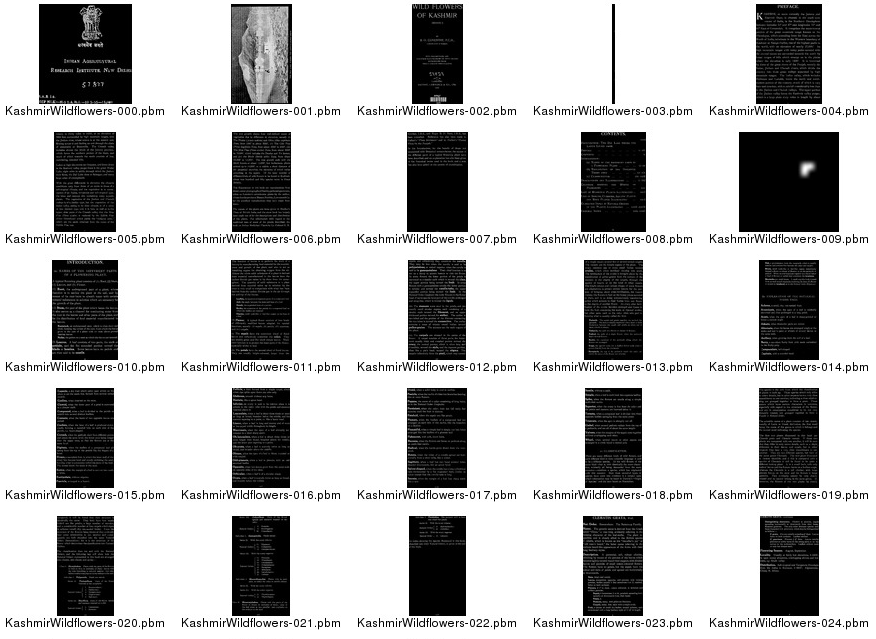
\includegraphics[scale=0.37]{Contact_sheet1.png}
\centering
\end{figure}
\begin{Verbatim}[fontsize=\scriptsize]
[root@plainsong ~]# montage -verbose -label '%f' -define pbm:size=200x200 -geometry 100x100+38+6 -tile 5x images/*0??.pbm[100x100] images-contact.jpg
images/KashmirWildflowers-000.pbm[100x100]=>images/KashmirWildflowers-000.pbm PBM 864x928=>93x100 93x100+0+0 1-bit Bilevel DirectClass 0.070u 0:00.030
images/KashmirWildflowers-001.pbm[100x100]=>images/KashmirWildflowers-001.pbm PBM 1008x1664=>61x100 61x100+0+0 1-bit Bilevel DirectClass 0.130u 0:00.070
images/KashmirWildflowers-002.pbm[100x100]=>images/KashmirWildflowers-002.pbm PBM 864x1680=>51x100 51x100+0+0 1-bit Bilevel DirectClass 0.110u 0:00.059
...
images-contact.jpg PBM 880x2560 16-bit DirectClass 463KB 0.700u 0:00.570
[1]+  Done                    display -negate images/KashmirWildflowers-025.pbm
[root@plainsong ~]# display images-contact.jpg &
[1] 31008
\end{Verbatim}
\begin{figure}[!h]
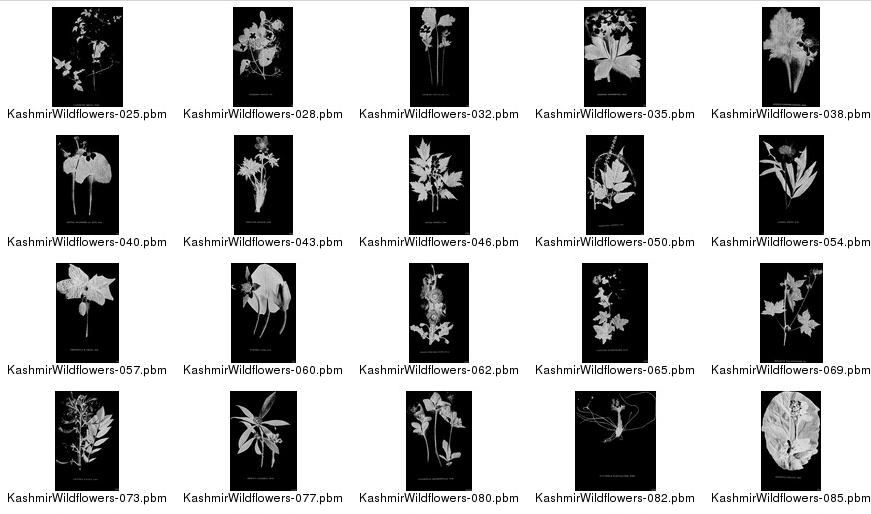
\includegraphics[scale=0.37]{Contact_sheet2.png}
\centering
\end{figure}
\begin{Verbatim}[fontsize=\scriptsize]
[root@plainsong ~]# filenums=(025 028 032 035 038 040 043 046 050 054 057 060 062 065 069 073 077 080 082 085 088 091 094 096 098)
[1]+  Done                    display images-contact.jpg
[root@plainsong ~]# for num in ${filenums[@]} ; do echo images/KashmirWildflowers-${num}.pbm ; done
images/KashmirWildflowers-025.pbm
images/KashmirWildflowers-028.pbm
images/KashmirWildflowers-032.pbm
...
[root@plainsong ~]# ls
anaconda-ks.cfg  images  images-contact.jpg  KashmirWildflowers.pdf  KashmirWildflowers.txt  pdftk-2.02-1.el6.x86_64.rpm
[root@plainsong ~]# mkdir flowerimages
[root@plainsong ~]# for num in ${filenums[@]} ; do cp images/KashmirWildflowers-${num}.pbm flowerimages/ ; done
[root@plainsong ~]# ls flowerimages
KashmirWildflowers-025.pbm  KashmirWildflowers-038.pbm  KashmirWildflowers-050.pbm  KashmirWildflowers-062.pbm  KashmirWildflowers-077.pbm  KashmirWildflowers-088.pbm  KashmirWildflowers-098.pbm
KashmirWildflowers-028.pbm  KashmirWildflowers-040.pbm  KashmirWildflowers-054.pbm  KashmirWildflowers-065.pbm  KashmirWildflowers-080.pbm  KashmirWildflowers-091.pbm
KashmirWildflowers-032.pbm  KashmirWildflowers-043.pbm  KashmirWildflowers-057.pbm  KashmirWildflowers-069.pbm  KashmirWildflowers-082.pbm  KashmirWildflowers-094.pbm
KashmirWildflowers-035.pbm  KashmirWildflowers-046.pbm  KashmirWildflowers-060.pbm  KashmirWildflowers-073.pbm  KashmirWildflowers-085.pbm  KashmirWildflowers-096.pbm
[root@plainsong ~]# montage -verbose -label '%f' -define pbm:size=200x200 -geometry 100x100+38+6 -tile 5x flowerimages/*.pbm[100x100] flowerimages-contact.jpg
flowerimages/KashmirWildflowers-025.pbm[100x100]=>flowerimages/KashmirWildflowers-025.pbm PBM 960x1344=>71x100 71x100+0+0 1-bit Bilevel DirectClass 0.100u 0:00.049
flowerimages/KashmirWildflowers-028.pbm[100x100]=>flowerimages/KashmirWildflowers-028.pbm PBM 976x1616=>60x100 60x100+0+0 1-bit Bilevel DirectClass 0.130u 0:00.060
flowerimages/KashmirWildflowers-032.pbm[100x100]=>flowerimages/KashmirWildflowers-032.pbm PBM 944x1600=>59x100 59x100+0+0 1-bit Bilevel DirectClass 0.120u 0:00.060
...
[root@plainsong ~]# display flowerimages-contact.jpg &
[1] 31041
[root@plainsong ~]# convert -negate flowerimages/*.pbm flowerimages.pdf
[1]+  Done                    display flowerimages-contact.jpg
[root@plainsong ~]# xpdf flowerimages.pdf 
\end{Verbatim}
So after all of this, there seemed to be no way to get pdftk to work with Centos 7, so I obliterated the OS and started over with Centos 6. After installing all the same packages, the downloaded rpm of pdftk finally took:
\begin{Verbatim}[fontsize=\scriptsize]
[root@plainsong ~]# wget https://www.pdflabs.com/tools/pdftk-the-pdf-toolkit/pdftk-2.02-1.el6.x86_64.rpm
--2015-11-25 06:49:17--  https://www.pdflabs.com/tools/pdftk-the-pdf-toolkit/pdftk-2.02-1.el6.x86_64.rpm
Resolving www.pdflabs.com... 23.253.106.249
Connecting to www.pdflabs.com|23.253.106.249|:443... connected.
HTTP request sent, awaiting response... 200 OK
Length: 1246631 (1.2M) [application/x-redhat-package-manager]
Saving to: ?pdftk-2.02-1.el6.x86_64.rpm?

100\%[==================================================================================================================================================================>] 1,246,631   2.87M/s   in 0.4s    

2015-11-25 06:49:18 (2.87 MB/s) - ?pdftk-2.02-1.el6.x86_64.rpm? saved [1246631/1246631]

[root@plainsong ~]# ls
anaconda-ks.cfg  install.log  install.log.syslog  pdftk-2.02-1.el6.x86_64.rpm
[root@plainsong ~]# rpm -Uvh pdftk-2.02-1.el6.x86_64.rpm 
Preparing...                ########################################### [100\%]
   1:pdftk                  ########################################### [100\%]
[root@plainsong ~]# pdftk KashmirWildflowers.pdf cat 3east output KashmirWildflowers-p003-rotated.pdf
[1]+  Done                    display flowerimages-contact.jpg
[root@plainsong ~]# xpdf KashmirWildflowers-p003-rotated.pdf 
Syntax Error (151154): Unknown segment type in JBIG2 stream
\end{Verbatim}
\begin{figure}[!h]
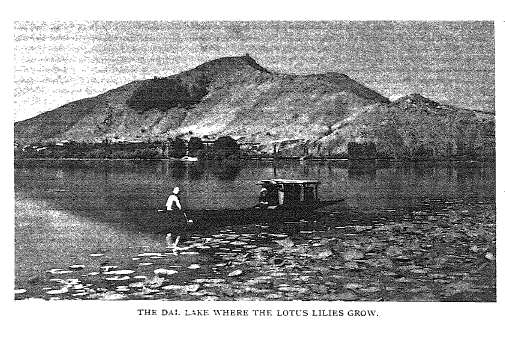
\includegraphics[scale=0.37]{rotated_pic.png}
\centering
\end{figure}
\begin{Verbatim}[fontsize=\scriptsize]
[root@plainsong ~]# pdftk KashmirWildflowers.pdf cat 230-233 output KashmirWildflowers-pp230-233-index.pdf
[root@plainsong ~]# xpdf KashmirWildflowers-pp230-233-index.pdf 
[root@plainsong ~]# pdftk KashmirWildflowers.pdf dump_data | less
PageMediaNumber: 37
PageMediaRotation: 0
PageMediaRect: 0 0 338.88 504.24
PageMediaDimensions: 338.88 504.24
PageMediaBegin
PageMediaNumber: 38
PageMediaRotation: 0
PageMediaRect: 0 0 338.88 504.24
PageMediaDimensions: 338.88 504.24
PageMediaBegin
PageMediaNumber: 39
PageMediaRotation: 0
PageMediaRect: 0 0 338.88 504.24
PageMediaDimensions: 338.88 504.24
PageMediaBegin
PageMediaNumber: 40
PageMediaRotation: 0
PageMediaRect: 0 0 338.88 504.24
PageMediaDimensions: 338.88 504.24
PageMediaBegin
PageMediaNumber: 41
...
[root@plainsong ~]# pdfinfo KashmirWildflowers.pdf
Keywords:       converted
Creator:        Adobe Scan-to-PDF Utility 4.0
Producer:       Adobe PDF Scan Library 4.1
CreationDate:   Thu Feb  2 15:31:26 2012
ModDate:        Thu Feb  2 15:31:43 2012
Tagged:         no
Pages:          234
Encrypted:      no
Page size:      338.88 x 504.24 pts
File size:      3945597 bytes
Optimized:      yes
PDF version:    1.6
root@plainsong ~]# pdftk KashmirWildflowers-pp230-233-index.pdf dump_data
InfoBegin
InfoKey: Creator
InfoValue: pdftk 2.02 - www.pdftk.com
InfoBegin
InfoKey: Producer
InfoValue: itext-paulo-155 (itextpdf.sf.net-lowagie.com)
InfoBegin
InfoKey: ModDate
InfoValue: D:20151125070012-07'00'
InfoBegin
InfoKey: CreationDate
InfoValue: D:20151125070012-07'00'
PdfID0: 2c144f87cd6af5ab884c954fa4104bbc
PdfID1: cc1d3666c933847bca95741fea163035
NumberOfPages: 4
PageMediaBegin
PageMediaNumber: 1
PageMediaRotation: 0
PageMediaRect: 0 0 338.88 504.24
PageMediaDimensions: 338.88 504.24
PageMediaBegin
PageMediaNumber: 2
PageMediaRotation: 0
PageMediaRect: 0 0 338.88 504.24
PageMediaDimensions: 338.88 504.24
PageMediaBegin
PageMediaNumber: 3
PageMediaRotation: 0
PageMediaRect: 0 0 338.88 504.24
PageMediaDimensions: 338.88 504.24
PageMediaBegin
PageMediaNumber: 4
PageMediaRotation: 0
PageMediaRect: 0 0 338.88 504.24
PageMediaDimensions: 338.88 504.24
[root@plainsong ~]# pdfinfo KashmirWildflowers-pp230-233-index.pdf
Creator:        pdftk 2.02 - www.pdftk.com
Producer:       itext-paulo-155 (itextpdf.sf.net-lowagie.com)
CreationDate:   Wed Nov 25 07:00:12 2015
ModDate:        Wed Nov 25 07:00:12 2015
Tagged:         no
Pages:          4
Encrypted:      no
Page size:      338.88 x 504.24 pts
File size:      78227 bytes
Optimized:      no
PDF version:    1.6
[root@plainsong ~]# pdftk KashmirWildflowers.pdf burst
[root@plainsong ~]# less doc_data.txt
[root@plainsong ~]# mkdir docpages
[root@plainsong ~]# mv pg*pdf docpages
[root@plainsong ~]# xpdf docpages/pg_0003.pdf &
[root@plainsong ~]# pdftotext docpages/pg_0006.pdf KashmirWildflowers-p006.txt
[root@plainsong ~]# less KashmirWildflowers-p006.txt
\end{Verbatim}
This does not work as the directions indicate, manual does not seem to state that there is a force option:
\begin{Verbatim}[fontsize=\scriptsize]
[root@plainsong ~]# echo -e "InfoKey: Title
> InfoValue: Wild Flowers of Kashmir
> InfoKey: Author
> InfoValue: Coventry, B. O.
> InfoKey: Keywords
> InfoValue: London,1923,Raithby Lawrence and Company" > KashmirWildflowers-metadata.txt
[root@plainsong ~]# pdftk KashmirWildflowers.pdf update_info KashmirWildflowers-metadata.txt output KashmirWildflowers-updated.pdf
pdftk Warning: InfoKey: (Title) already loaded when reading new InfoKey: (Author) -- skipping newer item
pdftk Warning: InfoValue: (Wild Flowers of Kashmir) already loaded when reading new InfoValue: (Coventry, B. O.) -- skipping newer item
pdftk Warning: InfoKey: (Title) already loaded when reading new InfoKey: (Keywords) -- skipping newer item
pdftk Warning: InfoValue: (Wild Flowers of Kashmir) already loaded when reading new InfoValue: (London,1923,Raithby Lawrence and Company) -- skipping newer item
root@plainsong ~]# pdftk KashmirWildflowers-updated.pdf dump_data
InfoBegin
InfoKey: Creator
InfoValue: Adobe Scan-to-PDF Utility 4.0
InfoBegin
InfoKey: Title
InfoValue: Wild Flowers of Kashmir
InfoBegin
InfoKey: Producer
InfoValue: Adobe PDF Scan Library 4.1
InfoBegin
InfoKey: Keywords
InfoValue: converted
InfoBegin
InfoKey: ModDate
InfoValue: D:20120202153143+05'30'
InfoBegin
InfoKey: CreationDate
InfoValue: D:20120202153126+05'30'
PdfID0: 3330d8ce27d89c4aae03ad5c36e495c3
PdfID1: 9df3695a3f8c1d468de3808a51dae798
NumberOfPages: 234
PageMediaBegin
PageMediaNumber: 1
PageMediaRotation: 0
PageMediaRect: 0 0 338.88 504.24
...
[root@plainsong ~]# pdfinfo KashmirWildflowers-updated.pdf
Title:          Wild Flowers of Kashmir
Keywords:       converted
Creator:        Adobe Scan-to-PDF Utility 4.0
Producer:       Adobe PDF Scan Library 4.1
CreationDate:   Thu Feb  2 15:31:26 2012
ModDate:        Thu Feb  2 15:31:43 2012
Tagged:         no
Pages:          234
Encrypted:      no
Page size:      338.88 x 504.24 pts
File size:      3998097 bytes
Optimized:      no
PDF version:    1.6
\end{Verbatim}
\end{document}
